\begin{comment}
comment from Manoj
Start with the properties of microservices and not directly Granularity? May be if we had talked about the qualities of microservices, it would have made more sense.
comment from Andrea
- compare the 'dimension by interface' and 'dimension by realization', and provide which should be considered
- define efficiency and reuse efficiency
- create a table to show what are good and bad services vs your goal and case.
- use common understandable term for 'volume' of service, either 'size'
To be done
- factors influencing size of a service such as single responsibility principle, technology, bounded context, autonomy
\end{comment}

\chapter{Granularity}\label{chapter:granularity}
In this chapter, the size of the microservices is discussed in detail. A major focus is to research various qualitative aspects which define the granularity of the microservices. Section \ref{section:granularity/principles} lists various principles which will guide architects to model the correct size by considering various aspects such as a) functionality b) data and c) business value. Furthermore, in Section \ref{section:granularity/dimensions}, various interpretations for defining the dimensions of the microservices are presented.Finally, the secion provides a complete picture of various factors which determine granularity.

\section{Introduction}\label{section:granularity/introduction}
The granularity of a service is often ambiguous and has different interpretations. In simple term, it refers to the size of the service. However, the size of a service itself can be vague. It cannot be defined as a single quantitative value because the concepts defining granularity are subjective in nature. For example, if we choose activities supported by the service to determine its granularity then we cannot have one single value. Instead, we have a hierarchical list of activities, where each activity can either refer to a) a simple state change, b) any action performed by an actor or c) a complete business process. \cite{Linthicum:2015aa}, \cite{Raf-Haesen:2015aa}
\\
Although, the interest upon the granularity of a component or service for the business users highly depends upon their business value, there is no doubt that the granularity affects the architecture of a system. The granularity of a service should reflect both the business perspective as well as the impact upon the overall architecture.
\\
The increase in size of a component or service is contributed by the level of the abstraction used. For example, in case of object oriented paradigm, the abstraction is chosen to represent the real world objects, each unit representing fine grained abstraction with some attributes and functionalities.
\\
Such abstraction is a good approach towards a) simplicity in development and b) easier understanding of the application. However, it is not always sufficient when high order business goals have to be implemented. It indicates the necessity of coarser-grained units than the units of object oriented paradigm. Moreover, the component based development introduces the concept of business components which target business problems and are coarser grained. Similarly, in service oriented architecture, the services provide access to the application and each application is composed of various component services. \cite{Linthicum:2015aa}

\section{Basic Principles of the Service Granularity}\label{section:granularity/principles}
In addition to the quantitative granularity, it is also helpful to address the qualitative aspects of granularity. The list below specifies some basic principles derived from various research papers and defines the qualitative properties of granularity. These principles will help architects to design microservices with the right granularity.

\begin{enumerate}
\item The correct granularity of a service is dependent upon the time. The various supporting technologies that evolve over time can be an important factor to define the level of decomposition. For eg: with the improvement in virtualization, containerization as well as platform as a service (\acrshort{PaaS}) technologies, it is fast and easy to automate deployment. These technologies makes it easy to support large number of services. Finally, the creation and operation of multiple fine-grained services is possible.\cite{Peter-Herzum:2000aa}

\item A good candidate for a service should be independent of the implementation but should depend upon the understandability of domain experts \cite{Raf-Haesen:2015aa, Peter-Herzum:2000aa}.

\item A service should be an autonomous reusable component and should support various cohesions such as functional cohesion (group similar functions), temporal cohesion (change in the service should not affect other services), run-time cohesion (allocate similar runtime environment for similar jobs; eg. provide same address space for jobs of similar computing intensity) and actor cohesion (a component should provide service to similar users).
\cite{Raf-Haesen:2015aa}, \cite{Peter-Herzum:2000aa}

\item A service should not support huge number of operations. In such case, any change in the service will affect large number of customers and there will be no unified and simplified view on the functionality. But, if the interface of the service is small, it will be easy to maintain and understand.\cite{Raf-Haesen:2015aa}, \cite{Pierre-Reldin:2007aa}

\item A service should provide transaction integrity and compensation. The functionalities supported by the service should be within the scope of one transaction. Additionally, the compensation should be provided when the transaction fails. If each operation provided by the service map to one transaction, then it will improve availability and fault-recovery. \cite{Raf-Haesen:2015aa}, \cite{Foody:2005aa} \cite{Bianco:2007aa}

\item The notion of right granularity is more important than that of fine or coarse. The size depends upon the usage condition and moreover depends on balancing various qualities such as reusability, network usage, completeness of context etc. \cite{Raf-Haesen:2015aa}, \cite{Lawrence-Wilkes:2004aa}

\item The level of abstraction of the services should reflect the real world business activities. The situation will help to map business requirements and technical capabilities easily. \cite{Pierre-Reldin:2007aa}

\item If there are ordering dependencies between operations, it can be easy to implement and test if the dependent operations are all combined into a single service \cite{Bianco:2007aa}.

\item There can be two better approaches for breaking down an abstraction. One way is to separate redundant data or data with different semantic meaning. The other approach is to divide services with limited control and scope. For example: A Customer Enrollment service which deals with registration of new customers and assignment of unique customer code can be divided into two independent fine-grained services: Customer Registration and Code Generation, each service will have limited scope and separate context of Customer.\cite{Pierre-Reldin:2007aa}

\item If there are functionalities 'A, B, C' provided by a service which are more likely to change than other functionalities 'D, E' in the service, it is better to extract the functionalities 'A, B, C' into a fine-grained service so that any further change on the functionalities will affect only limited number of consumers. \cite{Bianco:2007aa}
 
\end{enumerate}

\section{Dimensions of the Service Granularity}\label{section:granularity/dimensions}
As already mentioned in Section \ref{section:granularity/introduction}, it is not easy to define granularity of a service quantitatively. However, understanding granularity can be easier if we can project it along various dimensions, where each dimension is a qualifying attribute responsible for determining size of a service. Eventhough the  dimensions discussed in this section do not give the precise quantity to identify granularity, it definitely gives the hint to locate the service in granularity space. Moreover, it is interesting and beneficial to know how these dimensions come together for defining the size of the microservices.

\subsection{Dimensions given by Interface Perception of Consumers}\label{subsection:granularity/dimensions/interface}
One way to define the granularity is by understanding the perspective of the consumer towards the service interface. The various properties of the service interface responsible to define its size are listed below.
\begin{enumerate}
\item Functionality: It defines the amount of functionality offered by the service. The functionality can be either default functionality, which means some basic group of logic or operation provided by the service. Another type of the functionality can be parameterized and it can be optionally provided depending upon some values. Based on the scope of the functionality, the service can be either fine-grained or course-grained than the other services. Considering functionality criterion, a service offering basic \acrshort{CRUD} functionality is fine-grained than a service which is offers some data accumulation using orchestration. \cite{Raf-Haesen:2015aa}
\\
\item Data: It refers to the amount of data handled or exchanged by the service. The data granularity can be of two types. The first one is the input data granularity, which is the amount of data consumed or needed by the service in order to accomplish its tasks. The other type is ouput data granularity, which is the amount of data returned by the service to its consumer. Depending upon the size and quantity of business objects consumed or returned by the service interface, it can be coarse or fine grained. Additionally, if the business object consumed is composed of other objects rather than primitive types, then it is coarser-grained. For example: the endpoint "PUT customers/C1234" is coarse-grained than the endpoint "PUT customers/C1234/Addresses/default" because of the size of data object expected by the service interface. \cite{Raf-Haesen:2015aa}
\\
\item Business Value: According to \cite{Rolland:2015aa}, each service is associated with an intention or business goal and follows some strategy to achieve that goal. The extent or magnitude of the intention can be perceived as a metric to define granularity. A service can be either atomic or aggregate of other services. The level of aggregation is directly influenced by the target business goal of the services. An atomic service can have lower granularity than an aggregate in terms of business value. For example, sellProduct is coase-grained than acceptPayment, which is again coarse-grained than validateAccountNumber. \cite{Raf-Haesen:2015aa}
\end{enumerate}

\subsection{Dimensions given by Interface Realization}\label{subsection:granularity/dimensions/interface_realization}
The Section \ref{subsection:granularity/dimensions/interface} provides the aspect of granularity determined by the perception of customer to service interfaces. However, there can be different opinions on the same dimensions listed in Section \ref{subsection:granularity/dimensions/interface}, when it is viewed from the imlementation point of view. In this section, the same dimensions of granularity listed in the Section \ref{subsection:granularity/dimensions/interface} are analyzed again considering various aspects at implementation level.
\begin{enumerate}
\item Functionality: In Section \ref{subsection:granularity/dimensions/interface}, it is mentioned that an orchestration service has higher granularity than its constituent services with regards to the default functionality. If the realization effort is focused, it may only include compositional and/or compensation logic because the individual tasks are already accomplished by the constituent services. Thus, in terms of the effort in realizing the orchestration service it is fine-grained than from the view point of interface by consumer. \cite{Raf-Haesen:2015aa}
\\
\item Data: In some cases, services may utilize standard message format. For example: financial services may use \acrshort{SWIFT} for exchanging finanicial messages. These messages are extensible and are coarse grained in itself. However, all the data accepted by the service along with the message may not be required in order to fulfil the business goal of the service. In that sense, the service is coarse-grained from the viewpoint of consumer but is fine-grained in realization point of view. \cite{Raf-Haesen:2015aa}
\\
\item Business Value: It can make a huge impact when analyzing business value of service if the realization of the service is not considered well. For example: if we consider data management service which supports storage, retrieval and transaction of data, it can be considered as fine-grained because it will not directly impact the business goals. However, since other services are dependent on its performance, it becomes critical to analyze the complexity associated with the implementation, reliablity and the change in the infrastructure if needed. From the realization point of view, the data service is coarse-grained as compared to its consumer perspective. \cite{Raf-Haesen:2015aa}
\end{enumerate}

\begin{framed}
\textbf{\textit{Principle: A high value along functionality dimension of a microservices does not necessarily mean high business value for the microservice.}}
\\
It may seem that the dimensions: functionality and business value have direct proportional relationship. The business value of a service reflects business goals however the functionality refers to the amount of work performed by the service. A service to show customer history can be considered to have high value along functionality dimension because of the involved time period and database queries. However, it may be of a low business value to an enterprise. \cite{Raf-Haesen:2015aa}
\end{framed}


\subsection{R\textsuperscript{3} Dimension}\label{subsection:granularity/dimensions/r3}
Keen \cite{Keen:2015aa} and later  Weill and Broadbent \cite{Weill:1998aa} introduced a separate group of criteria to measure the granularity of a service. The granularity of a service is evaluated in terms of two dimensions as shown in the Figure \ref{fig:Reach-Range Model}

\begin{figure}[H]
\begin{center}
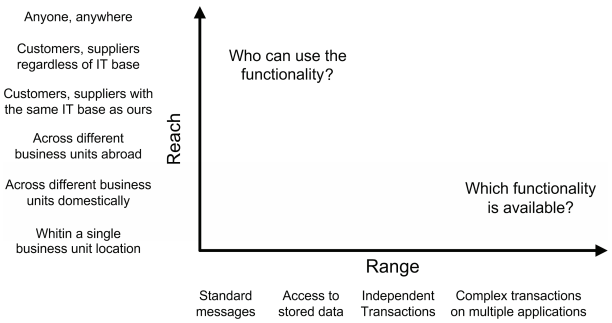
\includegraphics[width=0.8\textwidth]{figures/Granularity-R3-one}
\caption{Reach and Range model from \cite{Keen:2015aa, Weill:1998aa}}
\label{fig:Reach-Range Model}
\end{center}
\end{figure}

\begin{enumerate}
\item Reach: It provides various discrete levels to answer the question “Who can use the functionality? ” It provides the extent of consumers, who can access the functionalities provided by the service. It can be a customer, the customers within an organization, supplier etc. as shown by the Figure \ref{fig:Reach-Range Model}.
\\
\item Range: It gives answer to “Which functionality is available? ”. It defines the extent to which the information can be accessed from the service or shared with the service. The various levels of functionalities can be simple data access, transaction, message transfer etc as shown in the Figure \ref{fig:Reach-Range Model} The 'Range' measures the amount of data exchanged in terms of the levels of business activities important for the organization. One example of such activity levels with varying level of 'Range' is shown in Figure \ref{fig:Range Example}.

\begin{figure}[H]
\begin{center}
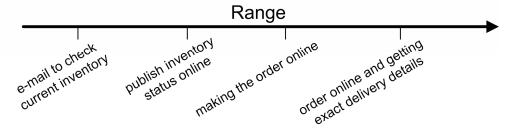
\includegraphics[width=0.8\textwidth]{figures/Granularity-R3-two}
\caption{Example to show varying 'Range' from \cite{Keen:2015aa, Weill:1998aa}}
\label{fig:Range Example}
\end{center}
\end{figure}

In the Figure \ref{fig:Range Example}, the level of granularity increases as the functionality moves from 'accessing e-mail message' to 'publishing status online' and then to 'creating order'. It is due to the change in the amount of data access involved in each kind of functionality. Thus, the 'Range' directly depends upon the level of data access.
\\
As the service grows, 'Reach' and 'Range' also peaks up, which means the extent of consumers as well as the kind of functionality increase. This adds complexity to the service. The solution proposed by \cite{Cockburn:2001aa} is to divide the architecture into services. However, only 'Reach' and 'Range' can not be enough to define the service. It is equally important to determine scope of the individual services. The functionality of the service is defined in two distinct dimensions 'which kind of functionality' and 'how much functionality'. So, this leads to another dimension of the service as described below.
\cite{Keen:2015aa, Weill:1998aa, Pierre-Reldin:2007aa}
\\
\item Realm: It tries to create a boundary around the scope of the functionality provided by the service. If we take the same example as shown by Figure \ref{fig:Range Example}, only 'range' defining the kind of functionaly such as creating online order does not explicitly clarifies about what kind of order is under consideration. The order can be customer order or sales order. The specification of 'Realm' defining what kind of order plays an important role here. So, we can have two different services each with same 'Reach' and 'Range' however different 'Realm' for customer order and Sales order.  \cite{Keen:2015aa, Weill:1998aa, Pierre-Reldin:2007aa}
\end{enumerate}

The consideration of all the aspects of a service including 'Reach', 'Range' and 'Realm' give us a model to define granularity of a service and is called R\textsuperscript{3} model. The volume in the R\textsuperscript{3} space for a service gives its granularity. A coarse-grained service has higher R\textsuperscript{3} volume than a fine-grained service. The Figure \ref{fig:R3 volume-granularity analogy greater}  and Figure \ref{fig:R3 volume-granularity analogy equal} show such volume-granularity analogy given by R\textsuperscript{3} model. \cite{Keen:2015aa, Weill:1998aa, Pierre-Reldin:2007aa}

\begin{figure}[H]
\begin{center}
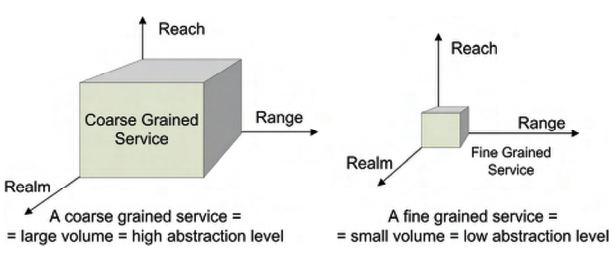
\includegraphics[width=0.8\textwidth]{figures/Granularity-R3-three}
\caption{R\textsuperscript{3} Volume-Granularity Analogy to show direct dependence of granularity and volume \cite{Pierre-Reldin:2007aa}}
\label{fig:R3 volume-granularity analogy greater}
\end{center}
\end{figure}

\begin{figure}[H]
\begin{center}
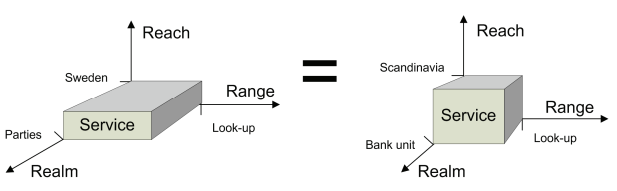
\includegraphics[width=0.8\textwidth]{figures/Granularity-R3-four}
\caption{R\textsuperscript{3} Volume-Granularity Analogy to show same granularity with different dimension along axes \cite{Pierre-Reldin:2007aa}}
\label{fig:R3 volume-granularity analogy equal}
\end{center}
\end{figure}
The Figure \ref{fig:R3 volume-granularity analogy greater} shows the use of R\textsuperscript{3} dimensions for comparing the size of the services. The service on the left side of the Figure \ref{fig:R3 volume-granularity analogy greater} has high abstraction level as well as high value for a) Reach, b) Range and c) Realm. However, the service on the right side has low abstraction level and has low value for a) Reach, b) Range and c) Realm. So, the service on the left side is a coarse grained service then the service on the right side of the figure.
Furthermore, the Figure \ref{fig:R3 volume-granularity analogy equal} depicts how R\textsuperscript{3} dimensions like a) Reach, b) Realm and c) Reach can be varied to control the size of the service. The service on the left side has different value of R\textsuperscript{3} dimensions than the service on the right side. However, both services have same volume and thus same value of granularity. It shows that the values along the three R\textsuperscript{3} dimensions managed in different ways as per the requirement to make the granularity as low as possible. 


\subsection{Retrospective}\label{subsection:granularity/dimensions/retrospective}
The Section \ref{subsection:granularity/dimensions/interface} and Section \ref{subsection:granularity/dimensions/interface_realization} divides granularity of a service along three different dimensions: data, functionality and business value. Moreover, the interpretations from the consumer's perspective and then the producer's viewpoint for realization are made.
Furthermore, the Section \ref{subsection:granularity/dimensions/r3} divides the aspect of granularity along a) Reach, b) Range, and c) Realm space. The granularity value of the service is given by the volume in the R\textsuperscript{3} space.
Despite it, the classification of granularity along data, functionality and business value does not provide discrete metrics to quantitatively define granularity. However, the given explanations and criteria are sufficient to compare granularity of two different services. These can be used to determine if a service is fine-grained than other service.
The R\textsuperscript{3} model in Section \ref{subsection:granularity/dimensions/r3} also provides various dimensions of granularity. This makes it easier to visualize the granularity and provides flexibility to compare the granularity of services.
\\
A case study to evaluate the impact of granularity on the complexity of the architecture using data, functionality and business criteria is presented in \cite{Pierre-Reldin:2007aa}. The study is performed at KBC Bank & Insurance Group of Central Europe. During the study, the impact of each kind of granularity was verified. The important results from the study are listed below.

\begin{enumerate}
\item A coarse-grained service in terms of 'Input Data' provides better transactional support, little communication overhead and also helps in scalability. However, there is a chance of data getting out-of-date quickly.
\item A coarse-grained service in terms of 'Output Data' also provides good communication efficiency and supports reusability.
\item A fine-grained service along 'Default Functionality' has high reusability and stability but low reuse efficiency.
\item A coarse-grained service due to more optional functionalities has high reuse efficiency, high reusability and also high stability but the implementation or realization is complicated.
\item A coarse-grained service along 'Business Value' has high consumer satisfaction value and emphasize the architecturally crucial points fulfilling business goals.
\end{enumerate}

Similarly, a study was carried out in Handelsbanken in Sweden, which follows the Service-Oriented architecture. The purpose of the study was to analyze the impact of R\textsuperscript{3} model on the architecture. It is observed that there are different categories of functionalities essential for an organization. Some functionalities can have higher 'Reach' and 'Range' with single functionality, while others may have complex functionality with low 'Reach' and 'Range'. The categorization and realization of such functionalities should be accessed individually. It is not necessary to have same level of granularity across all services or there is no one right volume for all services. However, if there are many services with low volume, then many services are additionally needed to accomplish high level functionalities. Furthermore, it increases interdependency among services and network complexity. Finally, the choice of granularity is completely dependent upon the IT-infrastructure of the company. The IT infrastructure decides which level of granularity it can support and how many of them. \cite{Pierre-Reldin:2007aa}


\begin{framed}
\textbf{\textit{Principle: IT-infrastructure of an organization affects granularity.}} \label{principle:granularity/IT_infrastructure}
\\
The right value of granularity for an organization is highly influenced by its IT infrastructure. The organization should be capable of handling the complexities such as communication, runtime operation, infrastructure etc if they choose low granularity. \cite{Pierre-Reldin:2007aa}
\end{framed}

Additionally, it is observed that a single service can be divided into number of granular services by dividing across either 'Reach', 'Range' or 'Realm'. The basic idea is to make the volume as low as possible as long as it can be supported by IT-infrastructure. Similarly, each dimension is not completely independent from other. For example: if the dimension 'reach' of a service has to be increased from domestic to global in an organization then the dimension 'realm' of the functionality has to be decreased in order to make the volume as low as possible, keep the development and runtime complexities in check. \cite{Pierre-Reldin:2007aa}

\begin{framed}
\textbf{\textit{Principle: Keep the volume as low as possible.}}
\\
If supported by IT-infrastructure, it is recommended to keep the volume of service as low as possible, which can be achieved by managing the values of a) Reach, b) Range, and c) Realm. It will help to decrease development and maintenance overload. \cite{Pierre-Reldin:2007aa}
\end{framed}

\section{Summary}\label{section:granularity/problem_statement}
In this chapter, various qualitative aspects related to the granularity of the microservices are analyzed. The interesting thing to notice is the various dimensions of the size across data, functionality and business value. However, it is also necessary to look into the quantitative aspects of granularity. Additionally, the various principles listed in Section \ref{section:granularity/principles} points towards other quality attributes of microservices including coupling, cohesion etc. The granularity is not the only attribute which is important while modeling the microservices but there are also other quality attributes which affect the granularity and also influence the overall quality of the microservices. The next task is to study the various quality attributes affecting the microservices and to derive their quantitative metrics.

 